\chapter{Behaviors of a sequence of random variables}
\section{Toolbox review: inequalities in probability}
这一节是一个 review,
复习一些在 measure theory 中我们已经证明过,
在 probability theory 中经常用到的 inequalities.
\subsection{Markov's ineqaulity and Chebyshev's inequality}
\begin{theorem}{Markov's inequality}
对于一个 non-negative random variable \(X\) (即 \(X \geq 0\) a.s.), 
任取 \(t > 0\), 都有
\[
\bP(X \geq t) \leq \frac{\bE[X]}{t}
\]  
\end{theorem}
\begin{remark}
这是一个很直观的 geometric intuition:
如果 $t$ 是均值 $\mu$ 的 3 倍, 那么 $X$ 大于 $t$ 
的测度就不应该超过均值 $\mu$ 的 1/3; 否则, $X$ 的均值
就一定大于 $\mu$ 了 (即便其他地方的值都为 0).

它 imply 这样一个时期: 对于 density function, 只要我们知道这个 RV 的均值,
那么对于 density function 截取任意点后面的 tail, 我们总是能够给出一个 upper bound:

\begin{center}
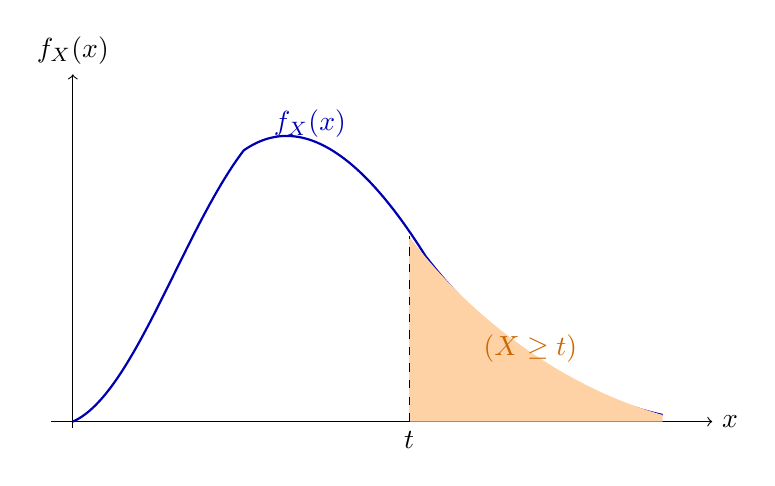
\begin{tikzpicture}[x=1.4cm,y=4.2cm]
  \draw[->] (-0.2,0) -- (5.8,0) node[right] {$x$};
  \draw[->] (0,-0.02) -- (0,1.05) node[above] {$f_X(x)$};

  % density curve
  \draw[thick, blue!70!black]
    (0,0)
    .. controls (0.55,0.08) and (1.0,0.58) .. (1.55,0.82)
    .. controls (2.15,0.96) and (2.75,0.74) .. (3.2,0.5)
    .. controls (3.8,0.24) and (4.55,0.08) .. (5.35,0.02);

  % tail shading
  \fill[orange!35]
    (3.05,0)
    -- (3.05,0.56)
    .. controls (3.5,0.36) and (4.3,0.12) .. (5.35,0.02)
    -- (5.35,0)
    -- cycle;

  % guide line at t
  \draw[dashed] (3.05,0) -- (3.05,0.56);

  % labels
  \node[below] at (3.05,0) {$t$};
  \node[orange!80!black] at (4.15,0.22) {$\bP(X\ge t)$};
  \node[blue!70!black] at (2.15,0.9) {$f_X(x)$};
\end{tikzpicture}
\end{center}


\end{remark}
\begin{proof}
我们考虑一个 indicator function $\mathbf{1}_{\{X \ge t\}}$, 这也是
一个 non-negative random variable. 
显然:
$$ 
X \geq t \cdot \mathbf{1}_{\{X \ge t\}}
 $$
 (在 $X \ge t$ 的事件上等于, 其他事件上小于), 并且这个 indicator function
 的 expectation 正是 $X$ 大于 $t$ 的概率 $\mathbb{P}(X \ge t)$. 
 
因而 by linearity of expectation,
 $$ 
 \mathbb{E}[X] \geq t \mathbb{E}[\mathbf{1}_{\{X \ge t\}}] = t \bP(X \ge t)
  $$
其值为 1 当 $X \ge t$ 时, 否则为 0.
    对于任意的 $t > 0$, 有
\end{proof}



\begin{corollary}{Chebyshev's inequality}
对于一个 random variable \(X\) 和任意的 \(t > 0\), 
如果它的方差 $\text{Var}(X)$ 是有限的, 那么
有
\[
\bP(|X - \bE[X]| \ge t) \le \frac{\text{Var}(X)}{t^2}
\]
\end{corollary}
\begin{remark}
Markov's ineq 是通过均值来 bound 非负随机变量
达到一定大小的概率 (在多少事件上是大于 $t$ 的);

Chebyshev's ineq 则是通过方差来 bound 任意随机变量
偏离均值达到一定程度的概率 (在多少事件上是偏离均值超过 $t$ 的).
\end{remark}
\begin{proof}
考虑 non-negative random variable $(X - \bE[X])^2$,
那么 
$$ 
\mathbb{P}(|X-\bE[X]| \ge t) = \mathbb{P}((X - \bE[X])^2 \ge t^2)
\leq \frac{\mathbb{E}[(X - \bE[X])^2]}{t^2} =
 \frac{\text{Var}(X)}{t^2}
 $$
\end{proof}

\subsection{Cauchy-Schwarz and Jensen's ineq}
\begin{theorem}{Cauchy-Schwarz inequality}
对于任意的 random variables \(X\) 和 \(Y\), 都有
\[
|\bE[XY]| \le \sqrt{\bE[X^2] \cdot \bE[Y^2]}
\]
\end{theorem}
这是 prob space 作为一个 measure space, 
其上的函数空间 
\(L^2(\Omega, \mathcal{F}, \bP)\) 
作为一个 Hilbert space, 自然的 Cauchy-Schwarz inequality.
不赘述了.

\begin{theorem}{Jensen's inequality}
对于一个 convex function \(\phi\) 和
任意的 random variable \(X\), 
只要 \(\bE[X]\) 和 \(\bE[\phi(X)]\) 都是 well-defined 的 (即 finite),
都有
\[
\phi(\bE[X]) \le \bE[\phi(X)]
\]
\end{theorem}
\begin{proof}
Let $x_0 := \bE[X]$.

Since \(\phi\) is convex, 
for any \(x\), there exists a supporting 
line to the graph of \(\phi\) at \(x\). 即
存在一个 $m\in \mathbb{R}$ s.t. 对于任意的 $y$, 都有
$$
\varphi(x) \geq \varphi\left(x_0\right)+m\left(x-x_0\right)
$$
因而 apply to $X$,
我们 a.s. 有
$$ \varphi(X) \geq \varphi(\mathbb{E}[X])+m(X-\mathbb{E}[X]) $$

因此 by linearity of expectation,
$$ 
\mathbb{E}[\varphi(X)] \geq \varphi(\mathbb{E}[X])+m(\mathbb{E}[X]-\mathbb{E}[X])=\varphi(\mathbb{E}[X])
$$
\end{proof}

\subsection{Fatou's Lemma, MCT and DCT}
我们在 measure theory 中最熟悉的三个定理. 复习一下.
这里不 prove 了. proof 请左转 measure theory notes.
\begin{theorem}{Fatou's Lemma}
令 \(\{X_n\}\) 是一列 non-negative random variables, 那么
$$ 
\bE[\liminf_{n\to\infty} X_n] \le
\liminf_{n\to\infty} \bE[ X_n] 
 $$
\end{theorem}
\begin{remark}
pointwise 下极限的积分, 
得到的结果不会大于每个函数积分的下极限.

因为 pointwise 下极限即:
 在每个 $\omega$ 上, 
 整个序列中最终稳定的最低水平
 , 这是最稳定的一层.

 而逐个函数可能会有一些 spike, 使得它的 expectation 很大,
 但是这个 spike 只出现有限次, 导致 pointwise limitinf
 的函数没有受到它的影响; 
 但是, 不同的 spike 可能 finitely 出现在不同的位置上, 
 而这个出现的行为是无限的(比如 typewritter 函数), 
 使得每个函数的 expectation 都很大, 
 从而导致 expectation 的 limit 很大.

 而 pointwise liminf 的 expectation 
 就是对每个点都取最终稳定的最低水平, 从而避免了这些 spikes 的影响.
\end{remark}

\begin{theorem}{Monotone Convergence Theorem (MCT)}
令 \(\{X_n\}\) 是一列递增的 non-negative random variables
(即 \(X_n \uparrow X\) a.s.), 那么
suppose $X:=\lim_{n\to\infty} X_n$ a.e. exists, 那么 a.s. 有
$$ 
\lim_{n\to\infty} \bE[X_n] = \bE[X]
 $$
\end{theorem}
\begin{remark}
如果 $X_n$ 是递减的, 那么 expectation 
的 limit 就等于逐点 limit 的 expectation 了.
\end{remark}


\begin{theorem}{Dominated Convergence Theorem (DCT)}
令 \(\{X_n\}\) 是一列 random variables, 
并且存在一个 a.e. pointwise limit \(X\) 
(即 \(X_n \to X\) a.s.), 
并且存在一个 integrable random variable 
\(Y\) 作为一个 bound: 使得 \(|X_n| \le Y\) a.s. 
对所有的 \(n\) 成立, 

那么
$$ 
\lim_{n\to\infty} \bE[X_n] = \bE[X]
 $$
\end{theorem}
\begin{remark}
只要这个序列有一个 integrable 的
uniform bound (不要有很多 unbounded 的 spike 就行了), 
那么 expectation 的 limit 就等于逐点 limit 的 expectation 了.
\end{remark}

\subsection{Tonneli and fubini}
\begin{theorem}{Tonneli's Theorem}
对于一列 non-negative random variables 
\(\{X_n\}\), 累加和积分(求期望)的顺序可以交换:
$$
\mathbb{E}\left[\sum_{n=1}^{+\infty} X_n\right]=\sum_{n=1}^{+\infty} \mathbb{E}\left[X_n\right]
$$
\end{theorem}

\begin{theorem}{Fubini's Theorem}
对于一列任意的 random variables \(\{X_n\}\),
只要其绝对值的 sum 的 expectation 是 finite 的 
(或者绝对值的 expectation 的 sum 是 finite 的,
by Tonneli 都是一样的),
那么就有 linearity of expectation 的推广:
$$
\mathbb{E}\left[\sum_{n=1}^{+\infty} X_n\right]=\sum_{n=1}^{+\infty} \mathbb{E}\left[X_n\right]
$$
\end{theorem}

\begin{remark}
Fubini 和 Tonelli 即: 
把 linearity of expectation 推广到 countable sum 的情况,
前提是 either 非负(因而无穷不用管) or 它们的 expectation 是一个绝对
收敛的 series 就行了.
\end{remark}

\section{Definition review: modes of convergence}
这一个 section 也是一个 review. 讲讲
不同的 convergence mode 的定义, 以及它们之间的关系.

首先, 我们对 pointwise limit 和 
uniform limit 的定义已经很熟悉了, 
这里就不赘述了.
(算了 uniform 还是提一嘴, 
意思是我们需要 pointwise limit 的
收敛速度也是 uniform 的, 
即对任意的 $\epsilon > 0$, 
都存在一个 $N$ 使得对于所有的 $n \ge N$ 
和所有的 $\omega$, 
都有 $|X_n(\omega) - X(\omega)| < \epsilon$,
是一个严格强于 pointwise 的收敛方式.
)

\begin{definition}{RV 序列的三种收敛方式}
\begin{itemize}
\item\textbf{ converge a.s. (almost surely) }
或称 converge with probability 1:
$$
\mathbb{P}\left(\lim _{n \rightarrow \infty} X_n=X\right)=1$$
即:
$$
\mathbb{P}\left(\left\{\omega \in \Omega: \lim _{n \rightarrow \infty} X_n(\omega)=X(\omega)\right\}\right)=1
$$
也就是说 $X_n$ 的 a.e. pointwise limit 是 $X$.

\item \textbf{converge in $L^p$}:
对于 $L^p$-integrable 的 random variables sequence $X_n$ 
和 $X$, 我们称 $X_n \xrightarrow{L^p} X$, 如果
$$
\lim _{n \rightarrow \infty} \mathbb{E}\left[\left|X_n-X\right|^p\right]=0
$$
即: 这个 seq of RVs 与这个 limit function 之间的
 $L^p$ distance 收敛到 0; 
 也就是它们的偏差 as a random variable,
 其 $p$-th moment 收敛到 0. 
\item  \textbf{converge in probability}:
对于任意的 $\epsilon > 0$, 如果
$$ 
\lim_{n\to\infty} 
\mathbb{P}(|X_n  - X| > \epsilon) = 0
$$
即 $X_n$ 与 $X$ 之间的偏差超过 $\epsilon$ 的概率收敛到 0.
\end{itemize}
\end{definition}




\section{Borel-Cantelli Lemma}









\section{Laws of Large Numbers}
\subsection{weak and strong LLN}
下面是概率论中最重要的定律之一: 
大数定律 (Laws of Large Numbers, LLN).

它证明的是一个十分符合直觉的结论: 
一个 random variable 的 sample mean 
(即 $n$ 个 i.i.d. 的 copy 的均值), 随着
sample 数量的增加, 会 converge to 它的 expectation.

就是说: 我们重复做一个相同的实验并
取结果的平均值, 当我们做的实验足够多时, 
这个平均值就会非常接近于这个实验的 
expectation, 也就是理论的均值. \\


例如最经典的例子就是抛硬币:
我们连续抛 $n$ 次一个公平的硬币, 
记录每次抛出正面 (记为 1) 或者反面 (记为 0),
然后计算这些结果的平均值, 随着 $n$ 的增加, 
这个平均值会趋近于 0.5, 等于
理论的 expectation (这是个 Bernouli random variable,
 expectation = $p$).\\

LLN 有两个阶段, weak LLN 和 strong LLN,
weak LLN 证明的是这个 convergence 是 in probability 的,
而 strong LLN 证明的是这个 convergence 是 a.s. 的.
就是说 strong LLN 是严格强于 weak LLN 的. 

\begin{theorem}{weak Law of Large Numbers}
\label{weak Law of Large Numbers}
对于一列 i.i.d. 的 random variables \(\{X_i\}\),
只要这个 random variable 的 expectation 是 finite 的
$\mathbb{E}[X_1^2] < \infty$, 
那么就有:
$$ 
\frac{X_1 + X_2 + \cdots + X_n}{n} 
\overset{p}{\longrightarrow} \mathbb{E}[X_1]\quad \text{as   } n \to \infty
$$    
\end{theorem}
\begin{proof}
简写 $\mu:= \mathbb{E}[X_1]$, 
$S_n:= \frac{X_1 + X_2 + \cdots + X_n}{n}$ for each $n$.

Let $\varepsilon > 0$. It suffices 
to show: $\mathbb{P}(|S_n - \mu| > \varepsilon) \to 0$ as $n \to \infty$. 
By Chebyshev's inequality, we have

\begin{align*}
\mathbb{P}\left(\left|S_n / n-\mu\right|
>\varepsilon\right) 
&\leq 
 \frac{\text{Var}(S_n / n)}{\varepsilon^2}\\
& = \frac{1}{n^2 \varepsilon^2} \left( 
\sum_{n=1}^n \mathbb{E}[|X_i - \mu|^2] 
+2 \sum_{1 \leq i < j \leq n} 
\mathbb{E}[(X_i - \mu)(X_j - \mu)]
\right)
\end{align*}
notice: 由于每个 $X_i$ 都是 i.i.d. 的,
independence $\implies$ uncorrelatedness
$\implies \text{Cov}(X,Y) = \mathbb{E}[XY]
-\mathbb{E}[X]\mathbb{E}[Y] = 0$, 
 因而 $\mathbb{E}[(X_i - \mu)(X_j - \mu)] = 
 \mathbb{E}[(X_i - \mu)] \mathbb{E}[(X_j - \mu)] =
 0 \cdot 0 = 0$ for each $i \neq j$. 

因而
$$
\mathbb{P}\left(\left|S_n / n-\mu\right|>\varepsilon\right)
= \frac{1}{\varepsilon^2 n^2} \sum_{n=1}^n \mathbb{E}[|X_i - \mu|^2]
= \frac{1}{\varepsilon^2 n}
\cdot n \text{Var}(X_1)
\overset{n\to \infty}{\rightarrow} 0
$$
\end{proof}

\begin{theorem}{strong Law of Large Numbers}
在 weak LLN\ref{weak Law of Large Numbers} 
的相同条件 (其实可以更弱,
让 $E[X_1] < \infty$ 即可) 下, 
我们其实可以得到一个更强的结论:
$$
\frac{X_1+\ldots+X_n}{n} \xrightarrow{\text { a.s. }} \mathbb{E}\left[X_1\right], \quad \text { as } n \rightarrow \infty
$$
\end{theorem}
\begin{proof}
For simplicity,
我们不证明更弱的条件 ($E[X_1] < \infty$) 
下的 strong LLN 了. 只沿用相同的条件.

简写 $\mu:= \mathbb{E}[X_1]$,
$\sigma^2 := \text{Var}(X_1)$, 
$S_n:= \frac{X_1 + X_2 + \cdots +X_n}{n}$ for each $n$,
以及
$$
Y_n := 
\frac{S_n}{n} - \mu 
$$
我们将要证明: $Y_n \overset{a.s.}{\longrightarrow} 0$.

首先, 在 weak LLN 的 proof 中, 我们已经证明了:
$$ 
\mathbb{E}(Y_n) = 0, \quad \mathbb{E}[Y_n^2]
= \frac{\sigma^2}{n}
 $$

我们发现: 当我们只采样 $n^2$ indexed 
的时候, 它们的 expectation 的 sum 是 finite 的, 
by p-test 
(因为 $\sum_{n=1}^\infty \frac{1}{n^p}$ 收敛当且仅当 $p > 1$),
即:
$$ \mathbb{E}\left[\sum_{n=1}^{+\infty} Y_{n^2}^2\right]=\sum_{n=1}^{+\infty} \mathbb{E}\left[Y_{n^2}^2\right]=\sum_{n=1}^{+\infty} \frac{\sigma^2}{n^2}<\infty
 $$
 先考虑所有 $Y_n$ 都非负的 case.  
我们知道: expectation of 一个 
non-negative random variable 是 finite 的, 
就 imply 它是 a.e. finite 的. 
因而 
$$
\sum_{n=1}^{+\infty} Y_{n^2}^2<\infty \quad \text { a.s. }
 $$

因而
$$ 
\lim_{n\to\infty} Y_{n^2} = 0 \quad \text{a.s.}
 $$

意味把在 $1, 4, 9, 16...$ 这些 index 的 
$Y_i$ 求 average, 确实收敛到了 $\mu$.

而我们可以通过 squeeze theorem 得到 general case:
对于任意正整数 $k$, 总能找到一对平方数把它夹在中间. 
比如令 $n^2 < k < (n+1)^2$.

我们发现:
$$ \frac{S_{n^2}}{(n+1)^2} \leq \frac{S_k}{k} \leq \frac{S_{(n+1)^2}}{n^2} $$
notice:
$\frac{S_{n^2}}{(n+1)^2} = \frac{S_{n^2}}{n^2} \cdot \frac{n^2}{(n+1)^2}$, 
前向 converge to $\mu$, 后向 converge to 1,
因而 $\frac{S_{n^2}}{(n+1)^2}\to \mu$, 后面那个也同理. 
因而夹逼得到 $S_k/k \to \mu$. 从而得证.

General case: 
$$
X_n=\max \left\{X_n, 0\right\}-\max \left\{-X_n, 0\right\}=: X_n^{+}-X_n^{-}$$
因而
$$
\frac{X_1+\ldots+X_n}{n}=\frac{X_1^{+}+\ldots+X_n^{+}}{n}-\frac{X_1^{-}+\ldots+X_n^{-}}{n} \xrightarrow{\text { a.s. }} \mathbb{E}\left[X_1^{+}\right]-\mathbb{E}\left[X_1^{-}\right]=\mathbb{E}\left[X_1\right]
$$
得证. 
\end{proof}
\begin{remark}
我们要求 $\mathbb{E}[|X_1|]$ 是 finite 的,
或者 $\mathbb{E}[|X_1|^2]$ 是 finite 的,
并不是一个硬性的条件, 只是结果确实 converge to 
$\mathbb{E}[X_1]$ 这个 finite value 的条件. 

实际上在 $\mathbb{E}[X_1]$ infinite (等于 $\infty$ 或者
$-\infty$) 时, 
我们会得到这个 average 发散, 因而也是
和 $\mathbb{E}[X_1]$ 一样, 只不过不是 converge 而是 diverge. 

此处不证明了.
\end{remark}



\subsection{application: Monte Carlo methods}
任何利用 LLN 
来近似计算
一个 quantity 的方法, 都可以称之为 Monte Carlo 方法.

它的核心思想是: 
\begin{itemize}
    \item 选择一个随机变量, 其 expectation 等于我们要计算的 quantity.
    \item 大量重复采样这个随机变量, 并计算样本的平均值
    \item 根据大数定律, 这个平均值近似于我们要计算的 quantity.
    \item 我们可以用 Chebyshev's inequality 来给出这个近似的误差 bound.
\end{itemize}
\begin{example}{估算 $\pi$}
我们令 $X, Y \sim U([-1,1])$ 

那么 
$$ \mathbb{E}\left[\mathbf{1}_C(X, Y)\right]=\int_{-1}^1 \int_{-1}^1 \mathbf{1}_C(x, y) f_{X, Y}(x, y) d x d y=\frac{1}{4} \int_{-1}^1 \int_{-1}^1 \mathbf{1}_C(x, y) d x d y=\frac{\pi}{4} $$

注意我们每次随机采样 $X, Y$ 的时候, 
都是在 $[-1,1]\times [-1,1]$ 这个正方形里随机选一个点, 
即创建了一个 random variable 
$(X_i,Y_i)$ 并进行观测. 

根据 LLN, 不论单次的采样结果如何, 我们都可以得到
$$ 
\lim _{n \rightarrow \infty} \frac{\mathbf{1}_C\left(X_1, Y_1\right)+\ldots+\mathbf{1}_C\left(X_n, Y_n\right)}{n}=\frac{\pi}{4}, \quad \text { a.s. } 
$$

我们还可以用 Chebyshev's inequality 来给出这个近似的误差 bound:
$$
\mathbb{P}\left(\left|4 S_n / n-\pi\right|>\varepsilon\right) \leq \frac{\operatorname{Var}\left(4 S_n / n\right)}{\varepsilon^2}=\frac{4^2}{n^2 \varepsilon^2} \operatorname{Var}\left(\sum_{i=1}^n \mathbf{1}_C\left(X_i, Y_i\right)\right)=\frac{16}{n \varepsilon^2} \operatorname{Var}\left(\mathbf{1}_C\left(X_1, Y_1\right)\right) \approx \frac{1}{n \varepsilon^2}
$$
因而当 $n$ 足够大时, 几乎一定可以得到目标值.
\begin{python}
import random
def estimate_pi(n):
    S_n = 0 # This step 1
    for _ in range(n):
        # Here is step 2 (and 3)
        X = random.uniform(-1, 1)
        Y = random.uniform(-1, 1)
        # Check if the point is inside the unit circle
        if X**2 + Y**2 <= 1:
            S_n += 1
    pi_estimate = 4 * S_n / n
    return pi_estimate
# Example usage
n = 1000000
pi_approx = estimate_pi(n)
print(pi_approx)
\end{python}
\end{example}



\subsection{application: Bernstein Polynomials}


\subsection{application: Hypothesis testing}


